% Points in the input file are x-scaled by 0.5 so xval 1000 represents point 2000 in the original results. The reason for scaling was that TeX cannot handle > ~16k numbers
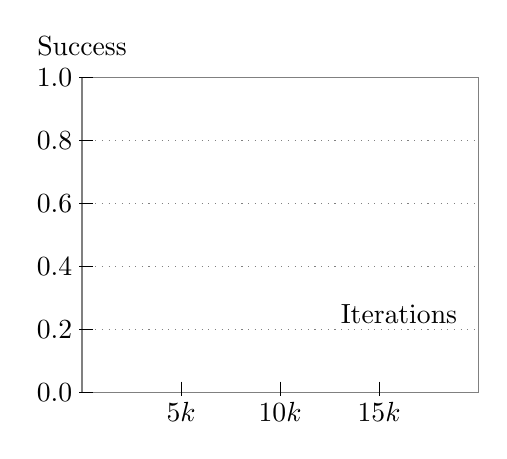
\begin{tikzpicture}[x=0.0005cm,y=4cm]
    % Draw the axes and grid lines
    \draw[-,gray] (0,0) -- (0,1) -- (10000,1) -- (10000,0) -- cycle; 
    \draw[-,gray,thin, dotted, ystep=0.2, xstep=10000] (0,0) grid (10000,1);
    \foreach \x in {2500, 5000, 7500}  \draw [-,xshift=0](\x,4pt) -- (\x,-1pt);
    \foreach \y in {0.0,0.2,0.4,0.6,0.8,1.0}  \draw [-,yshift=0](4pt,\y) -- (-1pt,\y);
    \foreach \x/\xtext in {2500/5k, 5000/10k, 7500/15k} \node at (\x,0) [below] {$\xtext$};
    \foreach \y/\ytext in {0.0,0.2,0.4,0.6,0.8,1.0}  \node at (0,\y) [left] {$\ytext$};
    \node at (0,1.1) {Success};
    \node at (8000,0.25) {Iterations};
    \draw[-,gray] plot[mark=o,mark size=3,mark options={color=black}] 
			file {data/hanoi5.CP.tikzdata};
    \draw[-,gray] plot[mark=x,mark size=4,mark options={color=black}] 
			file {data/hanoi5.CF.tikzdata};
\end{tikzpicture}
